\section{Evaluation}\label{sec:evaluation}
%\red{Aim of this section: •.}

%\red{Aim of this section: Brief introduction of what are we going to talk about in this section.}

% ns-3: https://www.nsnam.org/
In this section we conduct simulation based on realistic scenario trace file to verify the feasibility of our proposal. We decided to recreate the small public transport network of the UAB campus using the Network Simulator 3 (NS-3). NS-3 is a well-known discrete-event simulator targeted primarily for the research usage~\cite{ns-3-webpage}. We explain as well how the mobility model was obtained as well as what parameters were used during the simulation. Finally we will test our proposed method in the simulation to evaluate how it performs.

\subsection{Scenario: Campus buses}

%\red{Aim of this section: Explain a bit how the campus scenario works and how can be this useful in practice.}

In order to test our proposal we considered a very small public transportation network that works inside the Autonomous University of Barcelona (UAB) composed by 5 buses that makes different routes around the UAB campus. Is important to note that every single bus makes the same route daily. By this way, this example can be seen as a good example of deterministic networks.

Each bus has a DTN node that allows to achieve secret communications as well as source anonymity using onion routing protocol. There are several applications that can take profit of such networks like anonymous reporting systems.

\subsection{Mobility Model}

%\red{Aim of this section: explain how we get this scenario: open street maps -> sumo -> ns-3... }

We obtained the mobility model going through different stages. First, we exported the UAB Campus map from OpenStreetMaps into SUMO software~\cite{sumo}, filtering some unnecessary items like buildings and railways with the Java OpenStreetMap editor tool~\cite{josm}.

% bus-schedule: http://www.uab.cat/doc/horaris_busUAB_2015
Once the campus roads were imported in SUMO, we recreated the bus movements of each bus taking into consideration the official bus schedule of the UAB public transportation network \cite{bus-schedule}. In addition, we tuned some bus characteristics like acceleration and deceleration parameters in order to get coherent travel times.

%sumo-to-ns-2: http://www.ijarcsse.com/docs/papers/Volume_4/4_April2014/V4I4-0416.pdf
Finally, we exported the model to a NS-2 mobility trace as is explained in \cite{sumo-to-ns-2}. The NS-2 mobility trace can be used in NS-3. We used the simulator to obtain important contact related data of the campus network, i.e: information about the duration of the contacts as well as the instant of time when they occurred.

\subsection{Simulation setup}

%\red{Aim of this section: Explain and define the values used in the simulation itself as well as how we know that there is a neighbour able to contact with.}

% ns-3-dtn: https://www.nsnam.org/wiki/Current_Development
The DTN modules are under current development in NS-3 \cite{ns-3-dtn}. For this reason we decided to implement a neighbour discovery in the application layer. This application broadcasts beacons messages periodically looking for new contact opportunities. The interval time is the time to wait between beacons while the expiration time is the time a neighbour is considered valid, these parameters can be set up manually.

\begin{table}[h]
\centering
\begin{tabular}{l|l}
Parameter & Value \\
\hline
Number of nodes & 5 \\
Wi-Fi range & 100 meters \\
Interval time & 1 second \\
Expiration time & 2 seconds \\
Simulation time & 15 hours \\
DSS Rate & 1 Mbps \\
IEEE 802.11 specification & 802.11b
\end{tabular}
\caption{Simulation setup.}
\label{table:simulation-parameters}
\end{table}

As can be seen in table~\ref{table:simulation-parameters}, we also tuned different wireless parameters to be suitable with resource-constrained computers like those that could be used in each bus.

\subsection{Simulation results}

%\red{Aim of this section: Explain the results of this simulation. What we get explaining why.}

In figure~\ref{fig:contact-duration-group} we have an overall view of the network activity. There is a group that have really short contact times, these contacts can be suitable for those applications that does not require a huge amount of data to send. There is another group that has long contact times (nearly 7 minutes), these group is able to perform complex communications sending higher amount of data. The average contact time is near 1 minute indeed is suitable for several applications like anonymous reporting systems. A summary of contacts related information during the simulation is shown in table~\ref{table:contact-information}. With this simple network characterization we show that our evaluation model can be used for several applications. 

\begin{table}[h]
\centering
\begin{tabular}{l|l}
Metric & Value \\
\hline
Number of contacts & 1161 \\
Average contact time  & 72.72 seconds \\
Maximum contact time &  412 seconds\\
Minimum contact time &  1 second
\end{tabular}
\caption{Contact information.}
\label{table:contact-information}
\end{table}

\begin{figure}[hbt]
  \centering
  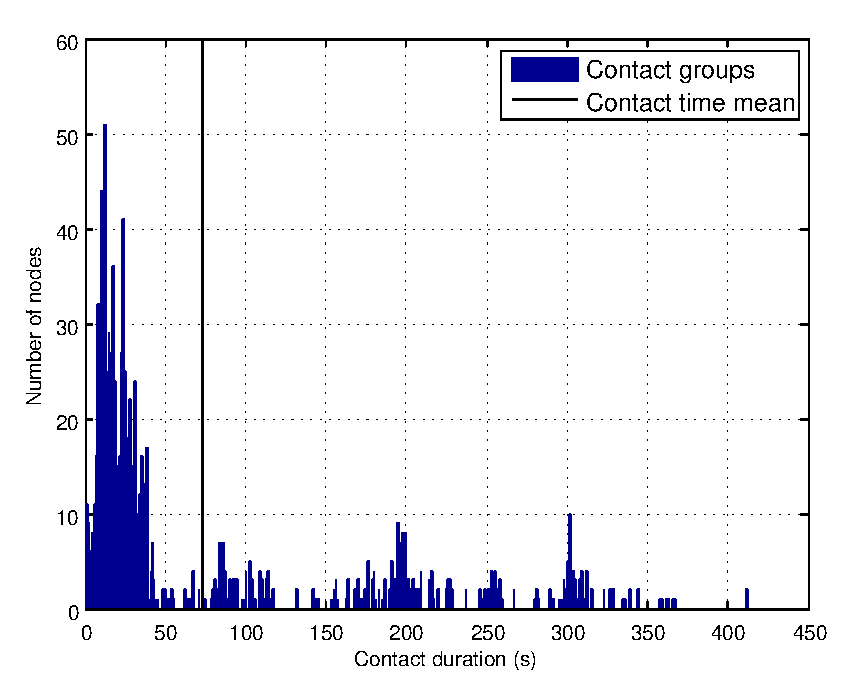
\includegraphics[scale=0.70]{imgs/statistics/contats-duration}
  \caption{Number of contacts with the same duration.}
  \label{fig:contact-duration-group}
\end{figure}


\red{Create a ratio between time and probability to guess the source. Normalize the value between 0 and 1. Do a 3-D graphic modifying k and n. Normalize like \url{https://docs.tibco.com/pub/spotfire/5.5.0-march-2013/UsersGuide/norm/norm_scale_between_0_and_1.htm}}